\documentclass[conference]{IEEEtran}
\IEEEoverridecommandlockouts
\usepackage{cite}
\usepackage{amsmath,amssymb,amsfonts}
\usepackage{graphicx}
\usepackage{textcomp}
\usepackage{xcolor}
\usepackage{booktabs}
\usepackage{multirow}
\usepackage{hyperref}
\usepackage{adjustbox}
\usepackage{array}
\usepackage{makecell}
\usepackage{tikz}
\usepackage{placeins}
\usepackage{float}
\usepackage{caption}
\usetikzlibrary{positioning, shapes.multipart, arrows.meta, calc}
\pagestyle{plain} % page numbers
\def\BibTeX{{\rm B\kern-.05em{\sc i\kern-.025em b}\kern-.08em
    T\kern-.1667em\lower.7ex\hbox{E}\kern-.125emX}}
\begin{document}

\title{MealVitals: Cloud-Native Dietary Management}
\author{
\begin{tabular}[t]{c}
\bfseries Christopher Terence Ng, Heng Yan Si, Poh Jia Jun\\
\{e1112601\textbar e0572838\textbar e0010964\}@u.nus.edu\\
\bfseries Tan Xue Ying, Thien Vui Chia, Zheng Zhiqing\\
\{e0313593\textbar e0818043\textbar e0293907\}@u.nus.edu
\end{tabular}
}

\maketitle

\begin{abstract}
One in three Singapore residents live with chronic hyperlipidemia or hypertension, a rate higher than the OECD average and one which remains stubbornly unchanged even as residents adopt healthier lifestyles post-COVID. We propose \textit{MealVitals}, a cloud-native Software-as-a-Service application that enables users to track nutritional intake, generate personalized meal plans, and produce grocery lists -- supporting every step of the dietary management journey.
\end{abstract}

%-----------------------------------------------------------------------
\section{Business Case}

\subsection{Context \& Problem Statement}

The 2024 National Population Health Survey~\cite{b1} conducted by the Ministry of Health (MOH) reports that approximately one in three Singapore residents live with hyperlipidemia or hypertension, despite a rise in the proportion of residents engaged in sufficient total physical activity from 75\% to 85\% since 2022. The same report also raises alarm at a rising obesity prevalence, and these figures present an opportunity to improve dietary management through technology-enabled nutrition tracking.

To date, MOH has actively promoted healthy living through a range of campaigns. Its initiatives~\cite{b2} primarily focus on:
\begin{enumerate}
    \item Increasing awareness of healthy living through community events and online resources.
    \item Helping residents make more informed choices through product labeling.
    \item Providing generic dietary recommendations (e.g.\ reducing sodium intake) through the Healthy~365 application.
\end{enumerate}

However, translating such campaigns into better-informed dietary choices remains a challenge. Chan et al.~\cite{b3} surveyed 955 Singaporeans and found substantial gaps in residents' knowledge of salt and sodium management:
\begin{enumerate}
    \item A majority were unaware of the recommended daily intake for salt (68\%) and sodium (83\%), and struggled to interpret sodium content across different serving sizes.
    \item Nearly one-third (30\%) of participants reported confusion when reading the Nutrition Information Panel.
\end{enumerate}

Consequently, residents frequently select food based on experience and common knowledge rather than on evidence-based labeling~\cite{b3}. Even when residents can correctly identify the healthier option, the cognitive effort required to apply this knowledge throughout the food consumption pipeline -- from meal planning to grocery shopping -- presents a significant barrier to adherence. A clear opportunity exists for a solution that simplifies dietary decision-making.

\subsection{Proposed Solution}

\textbf{MealVitals} addresses this gap by providing a cross-platform meal planning service that converts dietary constraints into personalized meal plans and grocery lists. \textbf{MealVitals} addresses two distinct market segments:
\begin{enumerate}
    \item The 1.1~million residents aged 18 and older diagnosed with or at risk of chronic conditions, who typically possess some nutritional knowledge but lack the tools to consistently make optimal dietary choices.
    \item Caregivers who plan meals on behalf of individuals with the aforementioned conditions.
\end{enumerate}

\textbf{MealVitals} generates personalized meal plans informed by health profiles, dietary constraints, and personal preferences, thereby improving adherence by simplifying meal planning and grocery purchasing. Studies~\cite{b4} have shown that elderly residents with chronic conditions often struggle with digital tools; \textbf{MealVitals} addresses this barrier by enabling a digitally proficient caregiver to plan meals on their behalf. Importantly, \textbf{MealVitals} provides dietary support rather than medical advice, which remains the responsibility of healthcare professionals.

%-----------------------------------------------------------------------
\section{Business Model}

\subsection{Overview}

\textbf{MealVitals} adopts a freemium model: all users receive access to core features for meal management and health monitoring at no cost, while advanced personalization capabilities -- such as automated meal plan generation and adaptive recommendations -- are reserved for premium subscribers. Table~\ref{tab:tiers} summarizes the feature set for each tier.

\begin{table}[H]
\caption{Feature Comparison by Tier}
\label{tab:tiers}
\begin{center}
\begin{tabular}{p{2.8cm}>{\centering\arraybackslash}p{2.2cm}>{\centering\arraybackslash}p{2.5cm}}
\toprule
\textbf{Feature} & \textbf{Free} & \textbf{Premium} \\
\midrule
Profile Limit & \multicolumn{2}{c}{Maximum of 5 profiles} \\
Health \& Dietary Filters & \checkmark & \checkmark \\
Meal Actions (swap, remove, favorite) & \checkmark & \checkmark \\
Grocery Cart \& Shopping List & \checkmark & \checkmark \\
Health Dashboard & \checkmark & \checkmark \\
Health Measurements Logging & \checkmark & \checkmark \\
Meal Selection & Pre-filtered by profile & Personalized recommendations \\
Meal Plan Creation & Manual & Automated (day/week) \\
\bottomrule
\end{tabular}
\end{center}
\end{table}

\subsection{Competitive Analysis}

\textbf{MealVitals} differentiates itself through two capabilities absent from competing products: constraint-based meal planning -- accounting for dietary restrictions, nutritional targets, user preferences, and recent consumption history -- and automated grocery list generation.

\textbf{MealVitals} does not currently offer dish recognition; however, integration with the FoodAI API~\cite{b5}, the same service integrated with Healthy~365, would enable rapid feature parity with competitors.

\begin{table}[H]
\caption{Competitive Landscape}
\label{tab:competitors}
\begin{center}
\begin{adjustbox}{max width=\columnwidth}
\begin{tabular}{lccccc}
\toprule
\textbf{Name} & \textbf{Fee} & \textbf{Dish Recog.} & \textbf{Nutr.\ Analysis} & \textbf{Meal Plan} & \textbf{Grocery} \\
\midrule
Healthy 365 (MOH) & Free & Yes & Yes & No & No \\
Food (NUS-ISS) & Free & Yes & Yes & No & No \\
Ventrickle & \$13/mo & Yes & Yes & No & No \\
\textbf{MealVitals} & \$9.90/mo & No & Yes & Yes & Yes \\
\bottomrule
\end{tabular}
\end{adjustbox}
\end{center}
\end{table}

\subsection{Cloud versus On-Premises Cost Comparison}

We recommend cloud deployment for three principal reasons: zero upfront capital expenditure, elastic scalability, and a lower total cost of ownership (TCO).

\subsubsection{Target Audience and Usage Projections}
The target audience of 1.1~million users is described in Section~I-B. Assuming a 2\% adoption rate over three years, the total addressable base reaches 22,000 users at full maturity. Uptake is projected to grow from 20\% in Year~1 (4,400~MAU) to 65\% in Year~2 (14,300~MAU), reaching 100\% by Year~3 (22,000~MAU).

We further assume that activity is concentrated within a 12-hour window corresponding to waking hours in Singapore's single time zone, with the remaining 12 hours largely idle.

\subsubsection{Cost Components and Assumptions}

\begin{itemize}
    \item\textbf{On-Premises Deployment:} Both Capital Expenditure (CAPEX) and Operating Expenditure (OPEX) are considered. CAPEX covers two server racks deployed in Singapore, depreciated over three years; Year~1 must be provisioned for the peak capacity projected in Year~3. OPEX includes electricity, broadband, and facility overheads.
    \item\textbf{Cloud Deployment:} As noted by Lenovo~\cite{b10}, cloud deployment incurs only OPEX through pay-as-you-go subscription fees. No upfront CAPEX is required.
\end{itemize}

Staffing costs are excluded from this analysis, as the project team operates under a start-up model.

\subsubsection{Three-Year Cost Comparison}

Cloud TCO is 28\% lower than on-premises over three years (Table~\ref{tab:tco}), driven primarily by the elimination of upfront capital expenditure. Monthly cloud cost scales with user growth, whereas an on-premises deployment must be provisioned for Year~3 peak capacity from the outset. Although the cloud's monthly cost eventually exceeds the on-premises monthly cost by Year~3, the cumulative three-year savings remain substantial.

\begin{table}[H]
\caption{Monthly On-Premises Cost}
\label{tab:onprem_monthly}
\begin{center}
\begin{tabular}{lr}
\toprule
\textbf{Component} & \textbf{Monthly Cost (\$)} \\
\midrule
CAPEX Amortization & 272 \\
Electricity & 96 \\
Broadband subscription & 150 \\
Maintenance and others & 50 \\
\midrule
\textbf{Total} & \textbf{568} \\
\bottomrule
\end{tabular}
\end{center}
\end{table}

\begin{table}[H]
\caption{Monthly Cloud Cost (Year~2)}
\label{tab:cloud_monthly}
\begin{center}
\begin{tabular}{lr}
\toprule
\textbf{Component} & \textbf{Monthly Cost (\$)} \\
\midrule
Compute -- Backend & 25 \\
Compute -- Website & 25 \\
Compute -- Recommender & 20 \\
Database & 323 \\
\midrule
\textbf{Total} & \textbf{393} \\
\bottomrule
\end{tabular}
\end{center}
\end{table}

\begin{table}[H]
\caption{Three-Year TCO Comparison}
\label{tab:tco}
\begin{center}
\begin{tabular}{lr}
\toprule
\textbf{Option} & \textbf{3-Year TCO (\$)} \\
\midrule
On-premises & 20,458 \\
Cloud & 15,180 \\
\bottomrule
\end{tabular}
\end{center}
\end{table}

\begin{table}[H]
\caption{On-Premises CAPEX Upfront Cost}
\label{tab:capex}
\begin{center}
\begin{tabular}{lr}
\toprule
\textbf{Component} & \textbf{CAPEX Cost (\$)} \\
\midrule
Compute (server) & 3,800 \\
Extra Storage & 2,000 \\
Network router & 2,000 \\
Power supply & 1,000 \\
Rack switches & 1,000 \\
\midrule
\textbf{Total} & \textbf{9,800} \\
\bottomrule
\end{tabular}
\end{center}
\end{table}

\FloatBarrier
%-----------------------------------------------------------------------
\section{Architecture \& Implementation}

\subsection{System Architecture \& Data Modeling}

\subsubsection{Application Design}
The application follows a three-tier architecture:
\begin{itemize}
    \item \textbf{Presentation layer} -- a React single-page application built with Vite and served over HTTPS.
    \item \textbf{Service layer} -- a FastAPI service exposing RESTful endpoints for authentication and business logic, running on Uvicorn.
    \item \textbf{Data layer} -- PostgreSQL for data storage.
\end{itemize}

\subsubsection{System Design}
The application is deployed on Google Cloud Platform (GCP), as illustrated in Fig.~\ref{fig:arch}:
\begin{itemize}
    \item \textbf{Cloud Storage} -- hosts the static website and stores Infrastructure-as-Code state files.
    \item \textbf{Cloud Run} -- provides serverless compute for API and authentication services; retrieves secrets from Secret Manager and builds from container images stored in Artifact Registry.
    \item \textbf{Cloud SQL} -- stores all application and authentication data.
\end{itemize}

\begin{figure}[H]
\centerline{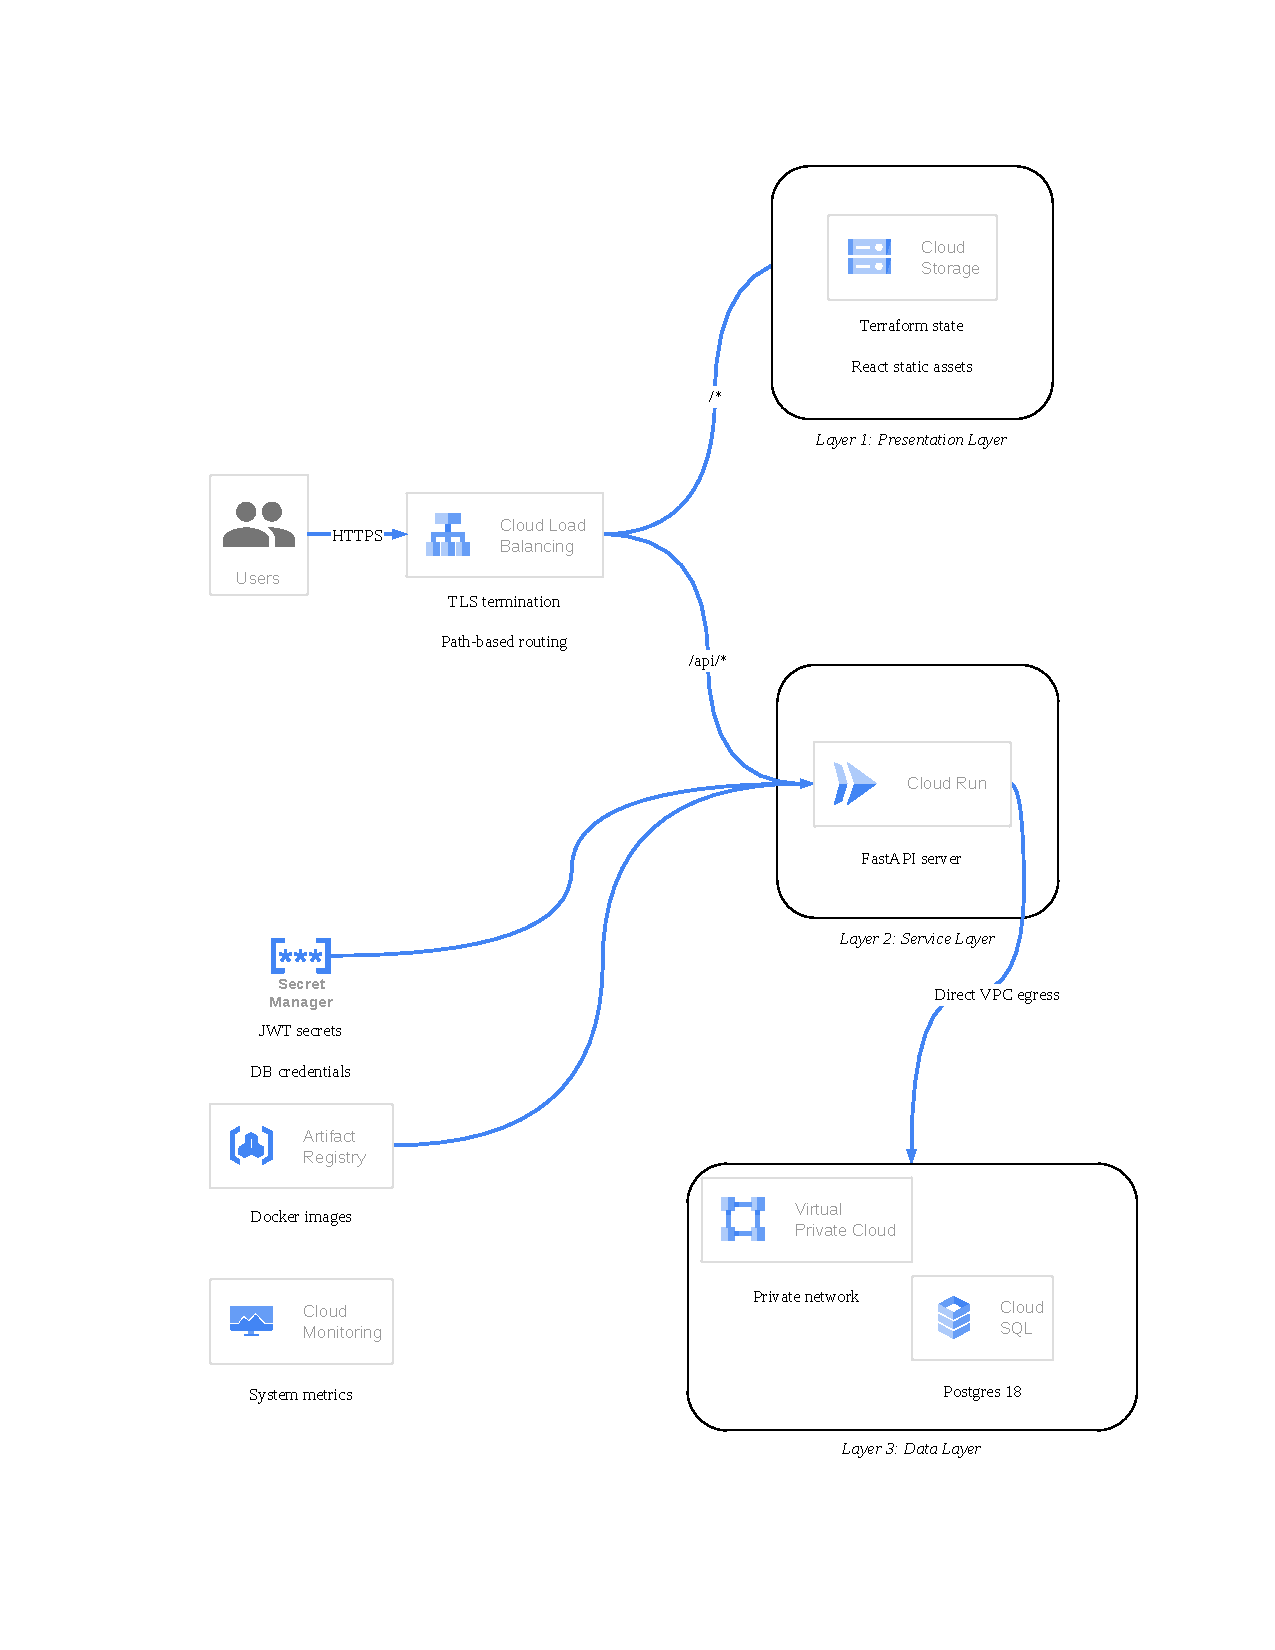
\includegraphics[width=\columnwidth]{architecture.pdf}}
\caption{System architecture}
\label{fig:arch}
\end{figure}

\subsubsection{Data Modeling}
The data model comprises the following entities:
\begin{enumerate}
    \item \textbf{Users} -- user accounts with demographic and dietary profile data.
    \item \textbf{Family Members} -- household members linked to a user or caretaker.
    \item \textbf{Caretakers} -- authenticated users who manage meals for family members.
    \item \textbf{Recipes \& Ingredients} -- dishes with nutritional information, sourced from MOH data.
    \item \textbf{Meal Plans} -- scheduled meal assignments across days and meal types.
    \item \textbf{Shopping Selections} -- aggregated ingredient selections for grocery lists.
    \item \textbf{Health Metrics} -- longitudinal health measurements (blood sugar, blood pressure, cholesterol).
    \item \textbf{Nutrient Thresholds} -- per-user nutritional targets used during plan generation.
\end{enumerate}


\subsection{Meal Recommendation Algorithm}

The meal recommender is built on \textit{Google OR-Tools CP-SAT}~\cite{b7}, a constraint programming solver that serves as the optimization engine. Premium users receive personalized meal recommendations accounting for dietary preferences, allergies, and health conditions. The recommender generates plans for breakfast, lunch, and dinner across time periods of one to seven days. Users may preserve previously accepted meals as fixed assignments and request recommendations only for remaining empty slots, enabling an interactive planning workflow. This formulation constitutes a constraint optimization problem~\cite{b6}. \textit{CP-SAT} is well suited because it natively handles binary and integer decision variables under both hard constraints and soft objective trade-offs.

\begin{table}[H]
\caption{Optimization Components}
\label{tab:optim}
\begin{center}
\begin{tabular}{p{1.8cm}p{5.8cm}}
\toprule
\textbf{Component} & \textbf{Description} \\
\midrule
Demand & Meal slots across 1--7 days for breakfast, lunch, and dinner \\
Supply & Candidate recipes with per-serving nutrient profiles, eligible meal types, and health-suitability labels \\
User constraints & Nutritional targets, dietary preferences, allergies, medical conditions, and thresholds specified at runtime \\
Pre-processing & Recipes violating allergy, diet, or medical suitability rules are filtered prior to optimization \\
\bottomrule
\end{tabular}
\end{center}
\end{table}

For each day~$d$, meal slot~$m$, candidate recipe~$r$, and nutrient type~$k$, the solver determines whether the recipe is selected and how many servings to assign. The daily nutrient total is computed as the sum of each selected recipe's per-serving nutrient value multiplied by its assigned servings.

The primary objective is to minimize deviation from the user's target intake, with emphasis on calories, protein, and carbohydrates. Secondary penalties discourage exceeding fat, sodium, and sugar targets; repeating recipes excessively; selecting cautionary dishes; and reusing recently served meals.

When nutrient thresholds are provided as runtime inputs, they override profile-derived defaults and are enforced as hard constraints. Structural feasibility constraints further ensure that each meal slot contains a valid number of dishes and that servings remain within permitted bounds.

\textit{CP-SAT} is preferable to simpler scoring-based approaches because it performs global optimization over the entire plan, simultaneously satisfying nutritional targets, dietary restrictions, preserved assignments, partial-week generation, dish-count limits, and variety constraints within a unified framework.

\subsection{System Interaction and Behavioral Design}

\textbf{MealVitals} supports four primary use cases: (1)~managing health profiles, (2)~generating meal plans, (3)~retrieving shopping lists, and (4)~tracking health metrics. Appendix~\ref{app:seq} presents detailed interaction sequences for user registration (Fig.~\ref{fig:seq_reg}) and the meal plan auto-fill flow (Fig.~\ref{fig:seq_meal}), which exercises the full stack from frontend through the CP-SAT solver.

\subsection{Security, Authentication and Secret Management}

\textbf{MealVitals} handles sensitive user data including email addresses, dietary preferences, allergies, and health-related profiles. As a multi-tenant SaaS platform, the system must ensure that only authenticated users can access the application and that each user's data is securely isolated. The security model follows the principle of defense-in-depth with five layers (Table~\ref{tab:security}).

\begin{table*}[htbp]
\caption{Security Model -- Five-Layered Defense}
\label{tab:security}
\begin{center}
\begin{tabular}{p{2cm}p{3.5cm}p{4.5cm}p{4.5cm}}
\toprule
\textbf{Stage} & \textbf{Purpose} & \textbf{Implementation} & \textbf{Rationale} \\
\midrule
1. Email Verification &
Ensures that registered accounts correspond to valid, reachable email addresses, thereby reducing fraudulent registrations &
One-time verification codes that are short-lived, single-use, and rate-limited; the account remains inactive until verification is complete &
Prevents mass registration with invalid addresses and establishes a trusted communication channel for password resets and notifications \\
\addlinespace
2. JWT Minting &
Provides stateless, token-based authentication suitable for a browser-based SPA &
Upon successful login, the backend mints a signed JWT containing user identity (\texttt{sub}) and expiry (\texttt{exp}) claims; signing keys are stored in GitHub Secrets and injected during CI/CD &
The JWT signing secret must be protected; its exposure would permit the forging of valid authentication tokens \\
\addlinespace
3. Request Handling &
Enforces authentication on all privileged endpoints before executing business logic &
A bearer token is required on every protected endpoint; Nginx enforces CORS by restricting allowed origins to the official frontend domain &
Guarantees that users maintain a valid session before accessing resources and prevents unauthorized cross-origin API requests \\
\addlinespace
4. Token Validation &
Verifies token integrity on every request -- confirming proper signature, valid expiry, and legitimate session &
Signature and expiry are checked per request by backend middleware; invalid or expired tokens return an appropriate error response &
Any modification to the token payload invalidates the cryptographic signature, ensuring that tokens cannot be tampered with or forged \\
\addlinespace
5. Authorization &
Restricts data access to the authenticated user's own records and explicitly linked household members &
The backend enforces resource-level access control server-side, as client-side restrictions alone are insufficient &
Provides strict per-user data isolation within the shared multi-tenant infrastructure \\
\bottomrule
\end{tabular}
\end{center}
\end{table*}

%-----------------------------------------------------------------------
\section{Evaluation}

\subsection{User Engagement \& Evaluation}

The growth of MealVitals is evaluated across three funnels: acquisition, retention, and monetization~\cite{b8}. Acquisition employs leading indicators to measure onboarding velocity. Retention uses engagement and guardrail metrics to monitor sustained usage. Monetization relies on lagging indicators to assess the health outcomes delivered to users. All metrics are collected through Google Analytics.

\textbf{North Star Metric:} Weekly count of users who generate at least one meal plan.

\subsubsection{Leading Indicators}
These metrics quantify the rate at which new users complete key onboarding milestones:
\begin{enumerate}
    \item \textit{Health Profile Completion} -- number of new users who complete their health profile within 24~hours of registration, measured weekly.
    \item \textit{First Meal Plan Generation} -- number of new users who generate a meal plan within 48~hours of registration, measured weekly.
    \item \textit{Meal Plan Acceptance \& Adjustment} -- weekly count of meal plans that are accepted or modified by users.
\end{enumerate}

\subsubsection{Engagement \& Guardrail Metrics}
These metrics monitor ongoing usage and detect early signs of user dissatisfaction:
\begin{itemize}
    \item \textit{E1. User Retention (30/60/90 days)} -- proportion of users who remain active (defined as having generated at least one meal plan in the preceding week) at 30, 60, and 90~days post-onboarding.
    \item \textit{E2. Recommendation Satisfaction} -- ratio of positive to negative ratings (thumbs-up/thumbs-down) on daily meal recommendations.
    \item \textit{G1. Meal Plan Rejection Rate} -- weekly count of meal plans rejected due to perceived incompatibility with a medically advised diet.
\end{itemize}

\subsubsection{Lagging Indicators}
These metrics assess long-term health value:
\begin{itemize}
    \item \textit{Improved Cardiometabolic Health} -- proportion of active users who report reduced cholesterol, lower blood pressure, or improved glycemic control after six months. Data is collected via a biannual survey distributed automatically through Google Cloud Scheduler.
\end{itemize}

Active monitoring of these metrics informs the type of product work~\cite{b9} required and enables timely interventions -- such as user surveys or focus group discussions -- when any metric falls below the desired threshold.

\subsection{System Performance Monitoring Plan}

User-facing metrics are meaningful only when the underlying system is operating reliably. Rather than configuring alerts manually through the GCP Console, Terraform~\cite{b11} is used to declare monitoring resources as code, ensuring that alert thresholds and dashboards are reproducible and resistant to configuration drift. The monitoring plan addresses three dimensions: availability, performance, and reliability.

\begin{table}[H]
\caption{Monitoring Resources}
\label{tab:monitoring}
\begin{center}
\begin{adjustbox}{max width=\columnwidth}
\begin{tabular}{p{4.2cm}p{4cm}}
\toprule
\textbf{Resource Type} & \textbf{Purpose} \\
\midrule
\texttt{uptime\_check\_config} & Uptime check every 60\,s \\
\texttt{alert\_policy} (error) & Alert when $\geq$5\% of API requests fail within any 60\,s window \\
\texttt{alert\_policy} (latency) & Alert when meal plan generation latency exceeds 5\,s for a single-day plan \\
\texttt{logging\_metric} & Log solver failures when the API returns an empty meal plan \\
\texttt{notification\_channel} & Email notification to the operations team upon policy violation \\
\texttt{monitoring\_dashboard} & Unified dashboard for availability, performance, and reliability \\
\bottomrule
\end{tabular}
\end{adjustbox}
\end{center}
\end{table}

%-----------------------------------------------------------------------
\section{Limitations and Recommendations}

\textbf{Data Coverage.} The current meal dataset is not contextualized to Singapore's culinary culture. Future work could incorporate local dishes by enabling community-contributed recipes, with AI used to estimate nutritional values from user-submitted images or text descriptions.

\textbf{Secondary Market.} MealVitals currently targets home cooks; however, a substantial proportion of Singaporeans prefer dining out. Extending the application to include a nearest hawker centre locator would improve relevancy for this demographic.

\textbf{E-Commerce Integration.} Future development could explore integration with local supermarket platforms (e.g.\ NTUC FairPrice) for direct checkout functionality, streamlining the journey from meal planning to grocery purchase.

\textbf{Solver Parallelization.} The meal recommender currently generates recommendations sequentially across days. Parallelizing the solver across independent day-partitions would improve generation latency and balance computational load under increasing user demand.

\textbf{Runtime Secret Management.} While the current approach of injecting secrets via CI/CD is substantially more secure than hardcoded credentials, adopting runtime retrieval from a dedicated cloud secret manager (e.g.\ GCP Secret Manager's client library) would further reduce the risk of secret exposure.

%-----------------------------------------------------------------------
\section*{Code Repository}
The source code is available at \url{https://github.com/davidvct/healthy_meal_planner}. Setup instructions are provided in the repository README.

\begin{thebibliography}{00}
\bibitem{b1} Ministry of Health, ``National Population Health Survey (NPHS) 2024 report,'' 2025. [Online]. Available: \url{https://www.moh.gov.sg/others/resources-and-statistics/national-population-health-survey--nphs--2024-report/}
\bibitem{b2} Health Promotion Board, ``HPB annual report 2024,'' 2025. [Online]. Available: \url{https://www.hpb.gov.sg/docs/default-source/annual-reports/hpb-annual-report-2024.pdf}
\bibitem{b3} C.~Chan \textit{et al.}, ``Understanding knowledge, attitudes and behaviours related to dietary sodium intake in a multi-ethnic population in Singapore,'' \textit{Public Health Nutrition}, vol.~26, no.~12, pp.~2802--2814, 2023.
\bibitem{b4} L.~Leong \textit{et al.}, ``Older adults' perspectives and experiences with digital health in Singapore: Qualitative study,'' \textit{JMIR Human Factors}, vol.~11, e58641, 2024.
\bibitem{b5} FoodAI, ``FoodAI -- Food image recognition,'' [Online]. Available: \url{https://foodai.org/}
\bibitem{b6} Google Developers, ``Constraint optimization,'' 2024. [Online]. Available: \url{https://developers.google.com/optimization/cp}
\bibitem{b7} Google Developers, ``CP-SAT solver,'' 2024. [Online]. Available: \url{https://developers.google.com/optimization/cp/cp_solver}
\bibitem{b8} Reforge, ``How to choose \& measure impactful North Star Metrics,'' 2022. [Online]. Available: \url{https://www.reforge.com/blog/north-star-metrics}
\bibitem{b9} Reforge, ``Product work beyond product-market fit,'' 2020. [Online]. Available: \url{https://www.reforge.com/blog/product-work-beyond-product-market-fit}
\bibitem{b10} Lenovo, ``On-premise vs.\ cloud: Generative AI total cost of ownership analysis (2025 Edition),'' 2025. [Online]. Available: \url{https://lenovopress.lenovo.com/lp2225.pdf}
\bibitem{b11} HashiCorp, ``Terraform provider for Google Cloud,'' [Online]. Available: \url{https://registry.terraform.io/providers/hashicorp/google/latest/docs}
\end{thebibliography}

\clearpage
\appendix
\section{Sequence Diagrams}
\label{app:seq}

\begin{center}
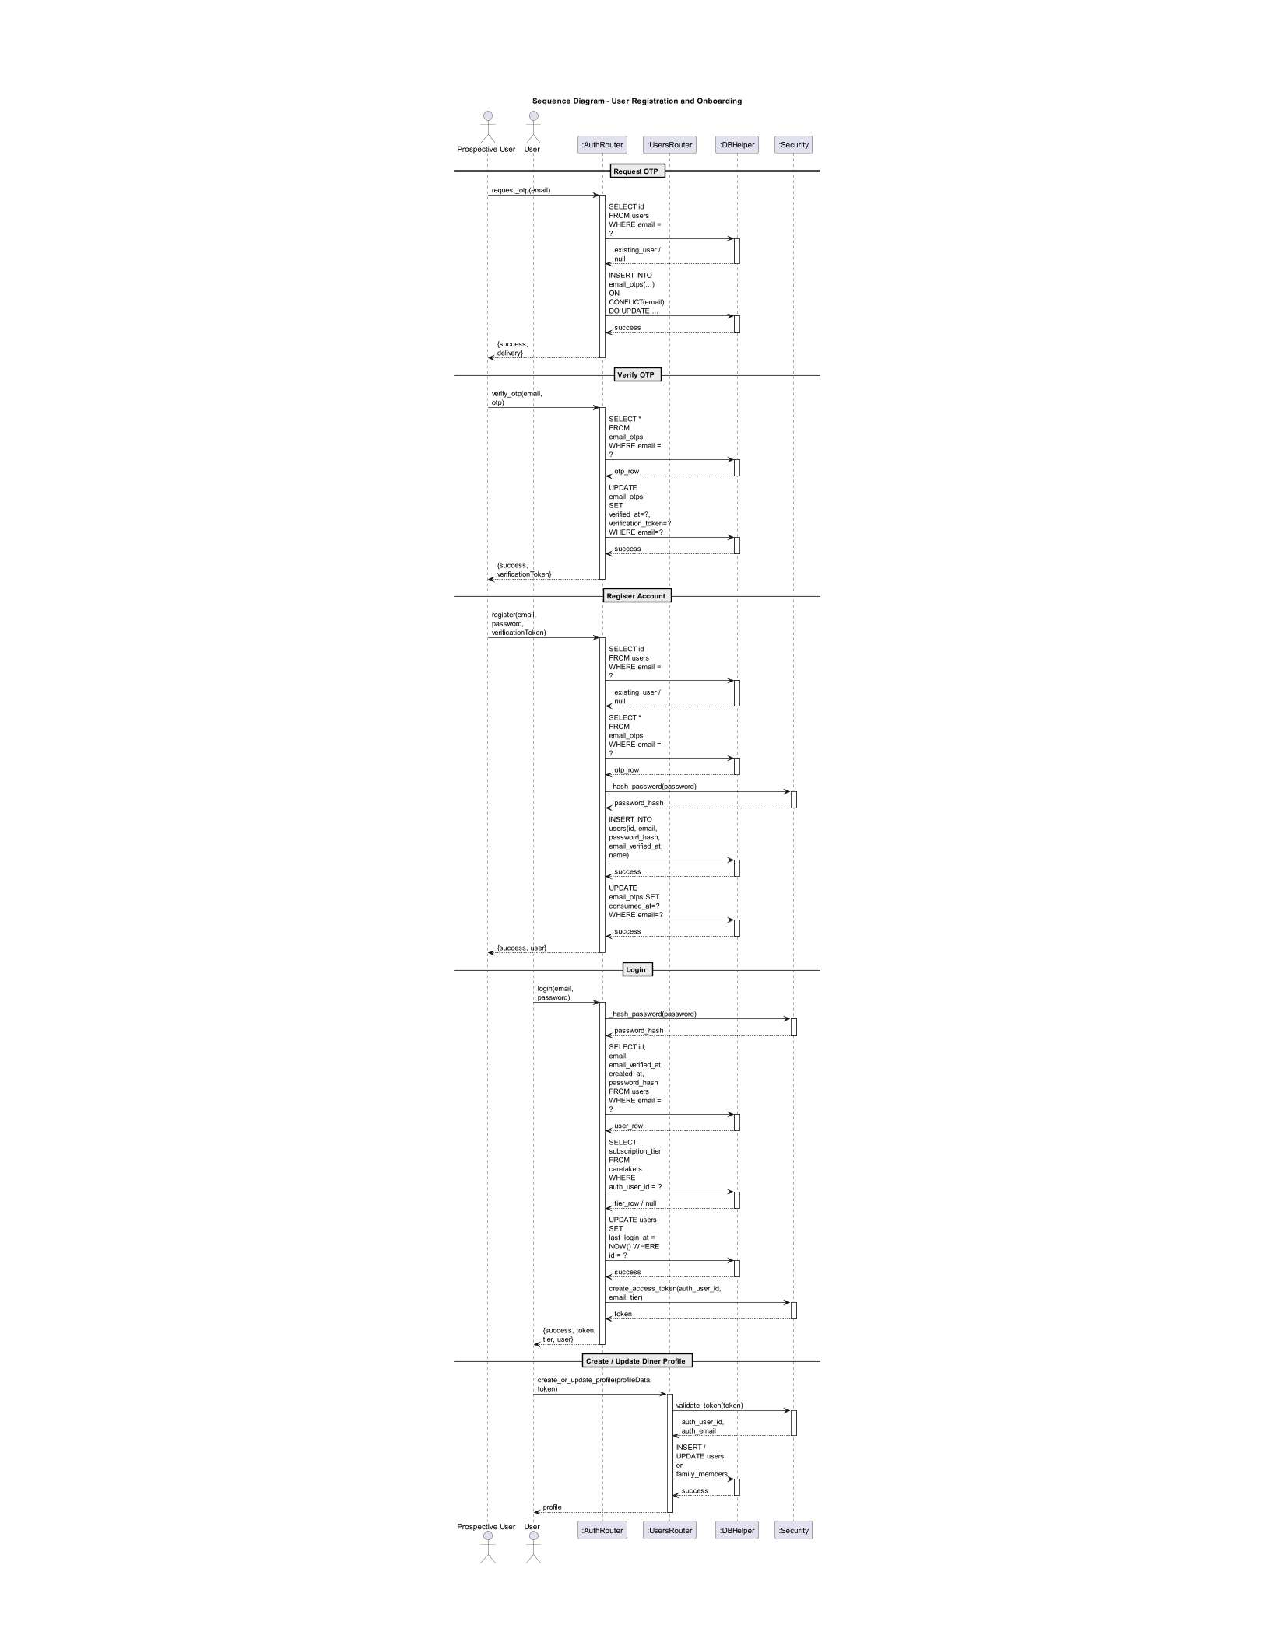
\includegraphics[width=\textwidth,height=0.85\textheight,keepaspectratio]{sequence_registration.pdf}
\captionof{figure}{User registration sequence}
\label{fig:seq_reg}
\end{center}

\clearpage
\begin{center}
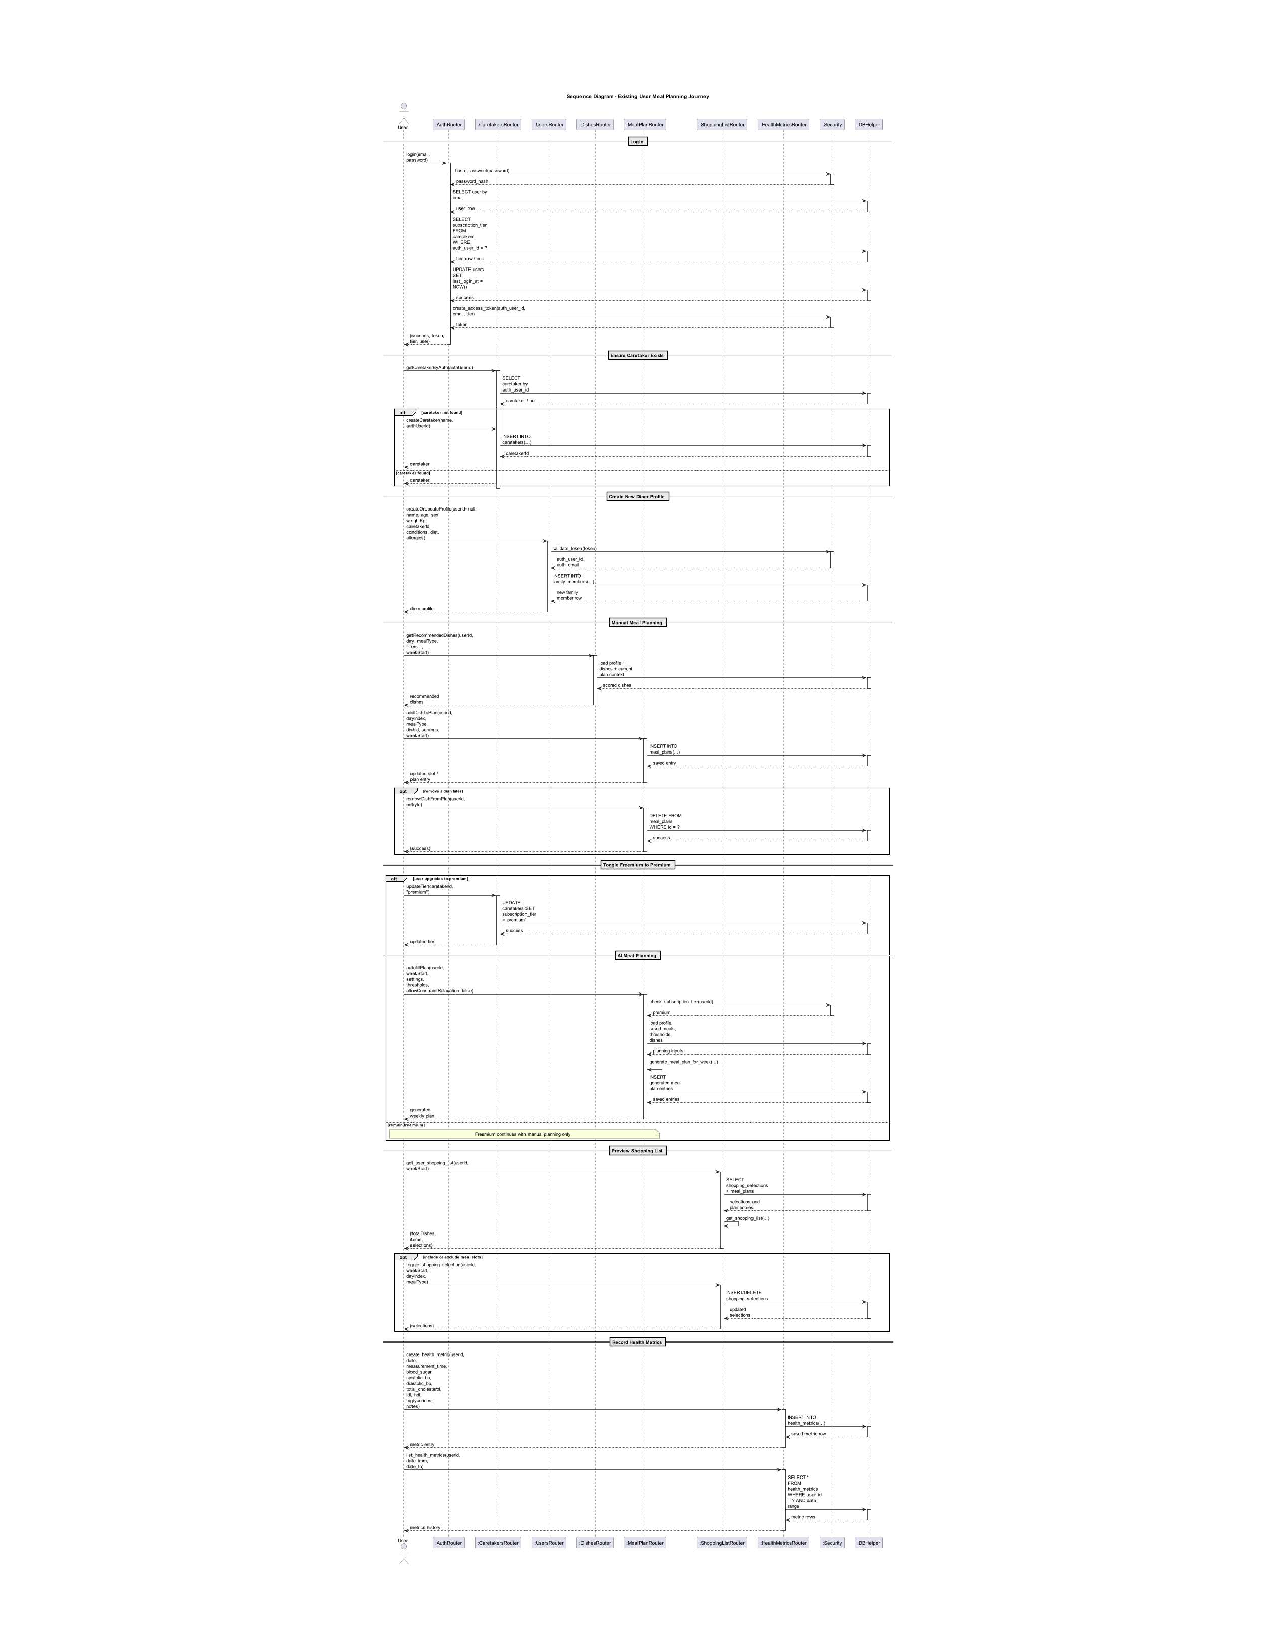
\includegraphics[width=\textwidth,height=0.85\textheight,keepaspectratio]{sequence_meal_planning.pdf}
\captionof{figure}{Meal plan auto-fill sequence}
\label{fig:seq_meal}
\end{center}

\end{document}
